\documentclass[titlepage, 12pt]{book}
\usepackage[spanish]{babel}

\pagestyle{plain}
\title{Falluto2.0 Un Model Checker para la verificaci\'on autom\'atica de sistemas tolerantes a fallas.}
\author{Raul Monti}
\date{Diciembre 2012}

\usepackage{graphicx} %para poner im\'agenes
\usepackage{float} % para establecer posici\'on de im\'agenes
\usepackage{amsmath} % para etiquetar flechas
\usepackage{tabularx}
\usepackage{enumerate}

\begin{document}

%TODO cambiar las palabras entre []
%TODO rellenar los '...'
\maketitle

\newpage
ACA VA EL RESUMEN
\newpage
ABSTRACT
\newpage
AGRADECIMIENTOS

\newpage
\tableofcontents

\newpage



\chapter{Introducci\'on}
\label{introduccion}

Es f\'acil notar la amplia dependibilidad que las personas hemos formado alrededor de dispositivos computacionales. A medida que crece la confianza hacia estos dispositivos para la realizaci\'on de diferentes tareas, crece tambi\'en el peligro que puede acarrear la ocurrencia de una falla en los mismos. En algunos casos, las actividades a las que son dedicados estos sistemas son actividades de bajo riesgo, como por ejemplo en un reloj de pulsera o un reproductor de m\'usica, y el incorrecto funcionamiento de los mismos no ocasiona da\~nos mayores. En otros casos las actividades realizadas son de car\'acter cr\'itico, como es por ejemplo en el caso de controladores de vuelo, o controladores de compuertas de contenci\'on fluvial. Es en estos \'ultimos donde el incorrecto funcionamiento del sistema puede provocar grandes [perdidas] monetarias y hasta llegar a ocasionar la [perdida] de vidas humanas.\\

Podemos considerar a la falla en una componente de hardware o software como una desviaci\'on de su funci\'on esperada. Las fallas pueden surgir durante todas las etapas de evoluci\'on del sistema computacional - especificaci\'on, dise\~no, desarrollo, elaboraci\'on, ensamblado, instalaci\'on- y durante toda su vida operacional\cite{faultInjection} (debido a eventos externos). Este comportamiento fuera de lo normal puede llevar a un falla funcional del sistema, provocando que se comporte de manera incorrecta, o simplemente deje de funcionar.\\
Es importante entonces, para lograr una mayor confiabilidad del software (confiabilidad de que se comporte como su especific\'on plantea) tomar acci\'on sobre la ocurrencia de estas fallas. Existen diferentes enfoques para tratar con fallas. Uno de ellos es elaborar sistemas tolerantes a fallas. A diferencia de otros enfoques en los que se busca eliminar o disminuir la ocurrencia de fallas, en estos sistemas se busca disminuir los efectos de las fallas y en el mejor de los casos recuperarse de estos y evitar que acarreen en fallas funcionales del sistema.\\

Queda claro entonces que un sistema tolerante a fallas provee grandes ventajas en comparaci\'on a uno que no contempla la ocurrencia de las mismas. Al igual que con el resto de los sistemas computacionales, es conveniente comprobar la correctitud de los sistemas tolerantes a fallas.
El dise\~no de algoritmos de tiempo real distribuidos tolerantes a fallas es notoriamente dificil y \emph{propenso a errores}: la combianaci\'on de la ocurrencia de fallas, conviviendo con eventos concurrentes, y las variaciones en las duraciones de tiempos reales llevan a una explosi\'on de estados que [genera una gran demanda] a la capacidad intelectual del dise\~nador humano\cite{SteinerRushby}.\\
En un mundo idealizado, los algoritmos son derivados por un proceso sistem\'atico conducido por argumentos formales que aseguran su correcci\'on respecto a la especificaci\'on original. En cambio, en la realidad contempor\'anea, los dise\~nadores suelen tener un argumento informal en mente y desarrollan el algoritmo final y sus par\'ametros explorando variaciones locales contra este argumento y contra escenarios que resalten casos dif\'iciles o problem\'aticos. La exploraci\'on contra escenarios puede ser parcialmente automatizada usando un simulador y prototipos \'agiles y esta automatizaci\'on puede llegar a incrementar el n\'umero de escenarios que ser\'an examinados y la confiabilidad de la examinaci\'on.\\ La examinaci\'on autim\'atica de escenarios puede ser llevada a un nivel a\'un m\'as avanzado usando \emph{Model Checking} \cite{SteinerRushby}.\\

En ciencias de la computaci\'on \emph{Model Checking} refiere al siguiente problema: dada una estructura formal del modelo de un sistema, y dada una propiedad escrita en alguna l\'ogica espec\'ifica, verificar de manera autom\'atica y exhaustiva si la el sistema satisface la propiedad. El sistema normalmente representa a un componente de hardware o software, y la f\'ormula a cumplirse representa una propiedad de \emph{safety} o \emph{liveness} que se desea verificar que el sistema cumpla, y de esta manera incrementar la confiabilidad sobre el mismo.
El reducido nivel de interacci\'on con el usuario de este m\'etodo es visto como un ventaja para la aplicaci\'on en la industria, ya que incrementa las posibilidad des ser usad por individuos no expertos\cite{RuysBrinksma}.\\
%TODO quiz\'as quitar esto y ponerlo en la seccion que sigue 
Sin embargo es preciso modelar el sistema y definir las propiedades, lidiando mientras tanto con el principal problema del Model Checking: \emph{la explosi\'on de estados} debido al incremento exponencial de los mismos a ra\'iz de la introducci\'on de variables en la especificaci\'on del sistema.\\

Es objetivo de este trabajo elaborar una herramienta que logre contribuir a disminuir los problemas al momento de verificar sistemas tolerantes a fallas. Por un lado se intenta evitar la introducci\'on de errores en el modelado del sistema en el que conviven fallas con procesos concurrentes. Por otro lado se busca evitar la introducci\'on excesiva de nuevas variables al representar el comportamiento de las fallas, evitando as\'i la nociva explosi\'on de estados al momento de la verificaci\'on.

Para ello presentamos la herramienta de model checking \emph{Falluto2.0}, orientada a la verificaci\'on de sistemas tolerantes a fallas. Esta herramienta presenta una capa de abstracci\'on sobre NuSMV\cite{NuSMV}, un model checker basado en diagramas de decisi\'on binaria. Falluto2.0 presenta un lenguaje de car\'acter declarativo para la introducci\'on de fallas en el modelado del sistema, generando un marco de seguridad contra la introducci\'on de errors evitando que el usuario deba explicitar el funcionamiento de la falla dentro del modelo.\\Este trabajo se presenta como extensi\'on tanto del trabajo realizado por Edgardo Hammes\cite{Falluto1} como del realizado por Nicol\'as Bordenabe\cite{Offbeat}.
%TODO seguir hablando del trabajo y poner la distribucion de los temas en el trabajo.





%%%%%%%%%%%%%%%%%%%%%%%%%%%%%%%%%%%%%%%%%%%%%%%%%%%%%%%%%%%%%%%%%%%%%%%%%%%%%%%%%%%%%%%%%%%%%%%%%%%%%%%%%%%%%%%%%%%%%%%%%%%%%%%%%%%%%%%%%%%%%%%%%%%%%%%%%%%%%%%%%%




\chapter{Tolerancia a fallas}

Mejorar la confiabilidad del sistema (el grado de confianza que se puede poner 
de manera justificada sobre el sistema) es usualmente presentado como el 
principal beneficio de la tolerancia a fallas. <Normalmente la confiabilidad es 
definida estad\'isticamente, indicando la probabilidad de que el sistema sea 
funcional y provea el servicio esperado en un alg\'un momento espec\'ifico >?
\cite{Felix}.




%..................................................................................................................................................................



\section{Fallas}
Intuitivamente, y dentro del contexto que nos competen, podemos definir a una falla como una desviaci\'on de su funci\'on esperada en una componente de hardware o software. Estas fallas pueden ocurrir en cualquier etapa de la evoluci\'on del sistema computacional en cuesti\'on -especificaci\'on, dise\~no, desarrollo, elaboraci\'on, ensamblado, e instalaci\'on- y durante toda su vida operacional\cite{FaultInject}.\\

Una definici\'on ligeramente m\'as formal nos sugiere definir el termino 'falla' basado en la observaci\'on de que los sistemas cambian su estado como resultado de dos clases de eventos muy similares: operaciones normales de sistema y ocurrencia de fallas. Por lo tanto, un falla puede ser modelada como una no deseada (pero sin embargo posible) transici\'on de estado en un proceso\cite{Felix}.



%..................................................................................................................................................................



\section{Sistemas tolerantes a fallas}
Existen sistemas dise\~nados para ser tolerantes a fallas: ellos o bien exhiben un bien definido comportamiento ante fallas cuando estas ocurren, o bien enmascaran la falla de la componente al usuario, es decir contin\'uan proveyendo su servicio est\'andar especificado a pesar de la ocurrencia de las fallas en la componente\cite{Cristian}.
Podemos entonces decir de manera vaga que la tolerancia a fallas es la habilidad que posee un sistema de comportarse de una manera bien definida ante la ocurrencia de una falla. En el momento de dise\~nar la tolerancia a fallas, un primer prerrequisito es especificar la clase de falla que ser\'a tolerada. Tradicionalmente esto se lograba usando como base alguno de los modelos de fallas est\'andares (crash, fail-stop, etc...), sin embargo puede hacerse de manera m\'as concisa especificando clases de fallas. El siguiente paso es enriquecer el sistema bajo consideraci\'on con componentes o conceptos que provean protecci\'on contra las fallas de una clase espec\'ifica\cite{FaultInject}.\\

En este trabajo podremos distinguir dos clases de fallas en particular. Un primer grupo de fallas es de tipo \textbf{permanente}: \'estas com\'unmente representan fallas reales causadas por problemas irreversibles en la componente. Una vez que una falla permanente ocurre, permanece activa y afectando al sistema durante el resto de su ejecuci\'on. Por otro lado, un segundo grupo de fallas se caracteriza por ser de duraci\'on instant\'anea. Afectan el estado del sistema en los puntos particulares de se ejecuci\'on en los cuales estas fallas ocurren, sin tener efectos permanentes sobre el mismo. Las mismas pueden repetirse indefinidamente durante la ejecuci\'on del sistema, permaneciendo activas solo en el momento en que afectan al sistema. Diremos que estas fallas son de clase \textbf{transient}.



%..................................................................................................................................................................



\section{Conclusi\'on}
En este trabajo entonces no realizaremos mayor diferencia formal entre transiciones buenas del sistema y transiciones debido a fallas, ambas ser\'an consideradas como transiciones posibles del sistema que podr\'an afectar o no el estado del mismo.\\

Distinguiremos adem\'as como dijimos dos clases de falla, las de tipo \textit{Permanente} y las de tipo \textit{Transient}.\\

Por \'ultimo, nos ocuparemos del modelado del sistema en general y nos centraremos en la inyecci\'on de las fallas en el mismo. No nos detendremos sin embargo en temas espec\'ificos al dise\~no de la tolerancia a las fallas.






%%%%%%%%%%%%%%%%%%%%%%%%%%%%%%%%%%%%%%%%%%%%%%%%%%%%%%%%%%%%%%%%%%%%%%%%%%%%%%%%%%%%%%%%%%%%%%%%%%%%%%%%%%%%%%%%%%%%%%%%%%%%%%%%%%%%%%%%%%%%%%%%%%%%%%%%%%%%%%%%%%





\chapter{Model Checking}

En el dise\~no de software y hardware de sistemas complejos, se consume m\'as tiempo y esfuerzo en verificaci\'on que en construcci\'on. Se entiende que la aplicaci\'on de t\'ecnicas reduce y aligera los esfuerzos en verificaci\'on a la vez que acrecientan su cobertura. Los m\'etodos formales ofrecen un gran potencial para obtener una integraci\'on temprana de la verificaci\'on en el proceso de dise\~no, para proveer de t\'ecnicas de verificaci\'on m\'as afectivas y reducir el tiempo invertido en aplicarlas\cite{prinMC}.\\

El \textbf{Model Checking} es un m\'etodo formal para la verificaci\'on exhaustiva de sistemas finitos. Logra esta verificaci\'on explorando todos los estados posibles del sistema con la intenci\'on de verificar la veracidad de una propiedad sobre el mismo.\\

En este cap\'itulo comenzaremos revisando algunos conceptos b\'asicos para entender el funcionamiento de los \textit{model checkers} (programas utilizados para la verificaci\'on mediante \textit{model checking}, y concluiremos presentando el proceso de \textit{model checking} junto con algunas caracter\'isticas de este m\'etodo.





%..................................................................................................................................................................




\section{Sistemas de transici\'on}
%TODO introducir sistemas de transicion

\subsection{Labelled transition systems - LTS}
Llamamos sistema de transiciones etiquetadas a un concepto de maquina abstracta usada en parte para el modelado de sistemas computacionales concurrentes. Este sistema de representaci\'on est\'a compuesto por un conjunto de estados, un conjunto de etiquetas o nombres, y una relaci\'on ternaria explicando las transiciones etiquetadas desde un estado hacia otro del sistema.\\
Formalmente podemos decir que un LTS es una tres-upla $M = (S,S_{0},L,R)$ donde:
\begin{itemize}
\item $S$ es un conjunto (de estados)
\item $S_0 \subseteq S$ es un conjunto de estados denominados iniciales
\item $L$ es un conjunto de etiquetas (nombres de transiciones)
\item $R \subseteq S \times L \times S$ es una relaci\'on ternaria (de transiciones etiquetadas)
\end{itemize}
Notemos entonces que si s1 y s2 son elementos en S, l es un nombre en L, y (s1,l,s2) pertenece a R, entonces estamos indicando que existe una transici\'on con nombre l desde el estado s1 al estado s2.\\
As\'i podemos modelar sistemas computacionales tomando cada elemento en S como un estado particular del sistema y definiendo relaciones etiquetadas entre los mismos para representar el comportamiento del sistema.\\

En particular nos interesa para este trabajo la capacidad que nos otorga este formalismo para representar sincronizaci\'on entre acciones de distintas componentes del sistema. En el ejemplo de la figura \ref{figura1} encontramos dos componentes, un productor y un consumidor, ambas con su representaci\'on LTS. Podemos a partir de ellas definir un sistema concurrente sincronizado en el cual las transiciones de igual nombre en cada componente deben ser ejecutadas de manera sincronizada, mientras que las transiciones propias de cada componente pueden ejecutarse independientemente. Vemos el sistema resultante en la figura \ref{figura2}. En ella la transici\'on punteada y etiquetada con 'Listo' representa la acci\'on sincronizada entre el productor y el consumidor. A su vez podemos ver en el estado punteado un caso de [interliving] entre los procesos sincronizados. All\'i podemos elegir entre darle paso a la acci\'on 'Producir' del productor, o dejar que el consumidor realice la acci\'on 'Consumir'. 


\begin{figure}[H] %Al incluir el paquete float, [H] obliga a posicionar la imagen justo en este lugar por mas que a latex no le guste.
  \centering
    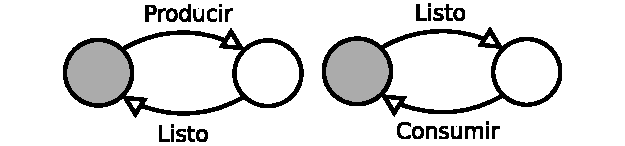
\includegraphics{Imagenes/prodYcons.pdf}
  \caption{El productor (izquierda) y el consumidor (derecha).}
  \label{figura1}
\end{figure}
~\\\\

\begin{figure}[H] %Al incluir el paquete float, [H] obliga a posicionar la imagen justo en este lugar por mas que a latex no le guste.
  \centering
    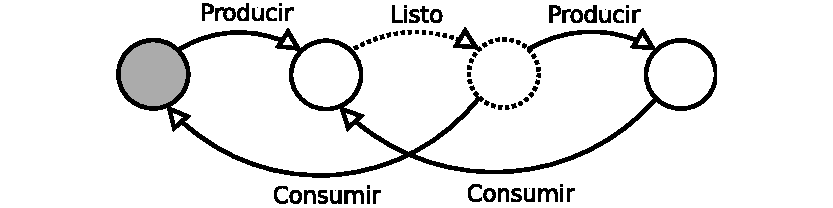
\includegraphics{Imagenes/prodYconsSincro.pdf}
  \caption{productor y consumidor de la figura \ref{figura1} sincronizados.}
  \label{figura2}
\end{figure}
~\\\\

\subsection{Estructuras de Kripke}
En model checking usamos un tipo de grafos de transici\'on de estados llamados \textit{Structuras de Kripke} para intuitivamente captar el comportamiento del sistema a modelar. Una \textit{estructura de Kripke} consiste en un conjunto de estados, un conjunto de transiciones entre esos estados, y una funci\'on que etiqueta cada estado con un conjunto de propiedades que son verdaderas en este estado. Los caminos en estas estructuras modelan la ejecuci\'on del sistema\cite{Clarke}. Estas estructuras son lo suficientemente expresivas como para captar aspectos de l\'ogicas temporales tales como (LTL y CTL) que interesan a la verificaci\'on de sistemas v\'ia model checking.\\

Formalmente podemos definir una estructura de Kripke como sigue\cite{Clarke}:\\

Sea AP un conjunto de proposiciones at\'omicas. Una estructura de Kripke M sobre AP es una cuatro-upla (S,$S_0$,R,L) tal que:
\begin{enumerate}
\item S es un conjunto finito de estados.
\item $S_0$ $\subseteq$ S es un conjunto de estados inciales.
\item R $\subseteq$ S x S es una relaci\'on de transici\'on que debe ser total, es decir, para cada estado s $\in$ S hay un estado s' $\in$ S tal que R(s,s').
\item L : S x $2^{AP}$ es una funci\'on que etiqueta cada estado con el conjunto de proposiciones at\'omicas verdaderas en ese estado.
\end{enumerate}
Una ejecuci\'on del sistema desde un estado s es representado en la estructura M como una secuencia infinita $\pi = s_0s_1s_2...$ tal que $s_0$ = s y $R(s_i,s_{i+1})$ vale para todo i $\geq$ 0.\\

Notemos que podemos traducir la representaci\'on LTS de un sistema a una representaci\'on en Estructuras de Kripke equivalente de la siguiente manera. Sea $M_1 = (S_1, S_{1_0} R_1, L_1)$ un sistema descripto en LTS, entonces construimos su descripci\'on $M_2 = (S_2,S_{2_0},R_2,L_2)$ en t\'erminos de estructuras de Kripke sobre AP de la siguiente manera:
\begin{itemize}
\item $ AP = \{action = e ~|~ e \in L_1 \cup \{null\}\} $
\item $ S_2 = S_1 \times (L_1 \cup \{null\}) $
\item $S_{2_0} = S_{1_0} \times \{null\}$
\item $R_2 = \{(s,a) \rightarrow (s',b) ~|~ s\overset{b}{\rightarrow}s' \in R_1, a \in L \cup \{null\}\}$
\item $L_2(s,a) = (action = a), ~\forall~(s,a) \in S_2$
\end{itemize}
Lo que hicimos fue entonces construir por cada estado $s_i$ y etiqueta $e$ en el LTS un estado en la estructura de Kripke que represente llegar al estado $s_i$ usando la etiqueta $e$. Dado que en el inicio de las ejecuciones no realizamos acci\'on alguna para llegar al estado inicial, es que hemos adem\'as definido para cada estado $s \in S_{1_0}$ un estado $(s,null)$ que lo represente en $S_2$. La funci\'on de relaci\'on se forma de manera intuitiva. El etiquetado indica qu\'e acci\'on se llev\'o a cabo para llegar a cada estado. Esto \'ultimo, junto con el nombre del estado, dejan en claro la transici\'on llevada a cabo en la ejecuci\'on del sistema definido en el LTS original. Vemos un ejemplo de traducci\'on LTS-Kripke en la figura \ref{ltsakripke}. Notemos que el sistema traducido puede ser depurado quitando estados no alcanzables como se muestra en la tercera figura de \ref{ltsakripke}.

\begin{figure}[H]
  \centering
    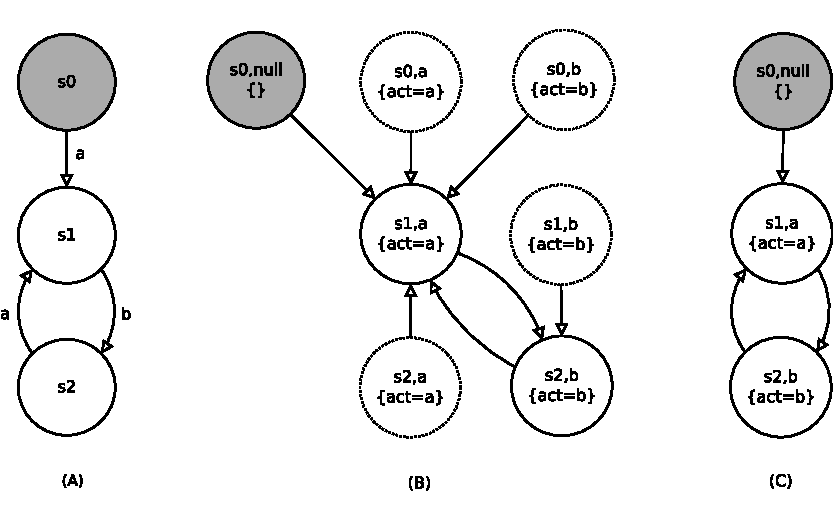
\includegraphics{Imagenes/ltsakripke.pdf}
  \caption{Ejemplo de traducci\'on de un sistema LTS a estructuras de Kripke. (A) El sistema en LTS; (B) El sistema en estructuras de Kripke; (C) El sistema en estructuras de Kripke depurado}
  \label{ltsakripke}
\end{figure}
~\\\\



%..................................................................................................................................................................



\section{De estructuras de Kripke a f\'ormulas \text{l\'ogicas}}
Si bien las estructuras de Kripke nos sirven para captar intuitivamente el comportamiento de los sistemas a modelar, los model checkers trabajan sobre el modelado del sistema en base a la l\'ogica de primer orden. A continuaci\'on veremos como lograr la interpretaci\'on de estructuras de Kripke usando f\'ormulas l\'ogicas de primer orden. En lo que a nosotros concierne, la l\'ogica de primer orden estar\'a comprendida por los conectivos l\'ogicos usuales - $\neg,\wedge,\vee,\rightarrow,etc...$ -, y haremos uso tambi\'en de los cuantificadores $\forall$ y $\exists$.\\

Supongamos que queremos modelar un sistema $P$, y tomemos todas sus variables de sistema $V = {v_0,v_1,...,v_n}$. Consideremos para el caso que todas estas variables toman valores de un domino finito $D$. Tenemos que una valuaci\'on de $V$ es una funci\'on total sobre el dominio, la cual asigna a cada variable en $V$ un valor en $D$. Notemos que dado que los valores de las variables del sistema son las que definen el estado del mismo en su totalidad, cada valuci\'on estar\'ia definiendo el estado del sistema. Por lo tanto en t\'erminos de estructuras de Kripke tenemos que si $M = (S,S_0,R,L)$ sobre $AP$ modela un sistema con variables en V entonces:
\begin{itemize}
\item $\textit{Usualmente } AP = \{v=d~|~ v \in V, d \in D\}.$
\item \textit{Cada estado s $\in$ S es una valuaci\'on sobre V.}
\item \textit{R explica la relaci\'on entre estas valuaciones, vale decir explica la transici\'on entre los cambios de valores en las variables del sistema.}
\item \textit{L(s) es el subconjunto de proposiciones en AP que son validas dada la valuaci\'on del estado s.}
\end{itemize}
Dada un estado en la estructura de Kripke, es decir una valuaci\'on $s:V\rightarrow D$, podemos escribir una f\'ormula sobre las variables en V tal que sea v\'alida solo para esta valuaci\'on\cite{Clarke}. La f\'ormula ser\'ia: $$(v_0 = s(v_0)) \& (v_1 = s(v_1)) \& ... \& (v_n = s(v_n))$$
Dado que en general una f\'ormula puede ser satisfecha por diferentes valuaciones, podemos a partir de ella definir el conjunto de estados que la satisfacen. Asi por ejemplo podemos definir una f\'ormula cuyos estados que la satisfacen sean solo los estados iniciales del sistema ($S_0$ en la estructura de Kripke que lo modela).\\

Adem\'as de definir los estados, necesitamos poder especificar tambi\'en transiciones como f\'ormulas interpretadas de primer orden. Para ello debemos lograr a partir de una f\'ormula representar la relaci\'on entre una valuaci\'on actual y la siguiente (estado actual y estado sucesor). Necesitaremos entonces otro conjunto de variables $V'$ el cual representen las variables en estado sucesor. De esta forma, dada la f\'ormula de transici\'on $F_r$ sobre el conjunto de variables $V \cup V'$ diremos que $s'$ es estado sucesor de $s$, es decir que $(s,s')\in R$, si y solo si $F_r$ es v\'alida al valuar todas sus variables en $V$ seg\'un $s$ y todas sus variables en $V'$ seg\'un $s'$.\\

Por \'ultimo, las proposiciones en AP nos permiten definir propiedades sobre los estados. Recordemos que las proposiciones at\'omicas en AP son de la forma $v=d$ con $v \in V$ y $d \in D$. Entonces tenemos que una proposici\'on $v=d$ es v\'alida en el estado $s$ si y solo si $d = s(v)$. En tal caso tenemos que $v=d \in L(s)$.




%..................................................................................................................................................................




\section{Representaci\'on de funciones booleanas en BDD}

Las funciones booleanas son un fuerte formalismo para representar los sistemas de transiciones y razonar acerca de propiedades sobre ellos. Se busca entonces poseer una eficiente representaci\'on de estas funciones para poder abarcar sistemas considerablemente complejos. NuSMV, como as\'i tambi\'en muchos otros model checkers, logra esta representaci\'on a partir de \textit{diagramas de b\'usqueda binaria}. Los BDD presentan muchas ventajas en cuanto a eficiencia en el c\'alculo y en el espacio de almacenamiento con respecto a otras representaciones como pueden ser las tablas de verdad o subclases de la formula proposicional como la forma normal conjuntiva.\\

Una funci\'on booleana de $n$ argumentos es una funci\'on $f : \{0,1\}^n \to \{0,1\}$. Podemos definir a los BDD como un subconjunto de grafos dirigidos ac\'iclicos finitos con las siguientes caracter\'isticas \cite{Huth}:
\begin{itemize}
\item Poseen un \'unico nodo inicial (un \'unico nodo al cual no llega ninguna arista).
\item Todas sus hojas son etiquetadas ya sea con '0' o con '1'.
\item Todos sus nodos que no son hojas est\'an etiquetados con el nombre de una variable booleana.
\item Cada nodo (excepto las hojas) posee dos aristas salientes hacia otros nodos del diagrama, una etiquetada con '0' y otra etiquetada con '1'.
\end{itemize}

Si B es un BDD entonces B define en sus hojas una \'unica funci\'on booleana sobre las variables en sus nodos de la siguiente manera: arrancando por el nodo inicial y dada una valuaci\'on $V=(v_1,v_2,...,v_n)$ sobre el conjunto de variables en los nodos, si $v_i$ es $0$ entonces tomo la arista saliente etiquetada con `0', de lo contrario tomo la etiquetada con `1'. Repito este paso en cada nodo hasta llegar a un hoja. El valor de la hoja es el valor, para esa valuaci\'on, de la funci\'on booleana representada.

Podemos reducir el tama\~no de los BDD logrando una mejora de eficiencia en el espacio de memoria necesario para la representaci\'on de las funciones booleanas. Para ello usamos los siguientes tres m\'etodos \cite{Huth}:
\begin{enumerate}[R1--]
\item \textbf{Remoci\'on de terminales duplicados.} Si el BDD posee m\'as de un nodo terminal '0', entonces redirigimos todas las aristas apuntando a esos nodos a unos solo de ellos y eliminamos el resto. Hacemos lo mismo con los nodos terminales '1'.
\item \textbf{Remoci\'on de verificaciones innecesarias.} Si ambas aristas salientes de un nodo $n$ apuntan a un mismo nodo $m$ entonces eliminamos el nodo $n$ redirigiendo todas sus arista entrantes al nodo $m$.
\item \textbf{Remoci\'on de no terminales duplicados.} Si dos nodos no terminales $n$ y $m$ son ra\'ices de subBDDs estructuralmente id\'enticos, entonces eliminamos uno de ellos y redirigimos todas sus aristas entrantes al otro.
\end{enumerate}
Estas reducciones no afectan la representaci\'on del BDD con respecto a la formula booleana original, y presenta una gran ventaja con respecto al espacio necesario para almacenar tablas de verdad por ejemplo. En la figura \ref{reduccionBDD} podemos ver un ejemplo de aplicaci\'on de estas reducciones. En la figura A vemos el BDD original, la figura B es el resultado de unificar las hojas seg\'un R1, la figura C es el resultado de eliminar uno de los nodos de etiqueta `y' tal como sugiere R3, y finalmente D es el resultado de aplicar la regla R2 eliminando el nodo de etiqueta `x'.

%TODO demasiado tonto el ejemplo?
\begin{figure}[H]
  \centering
    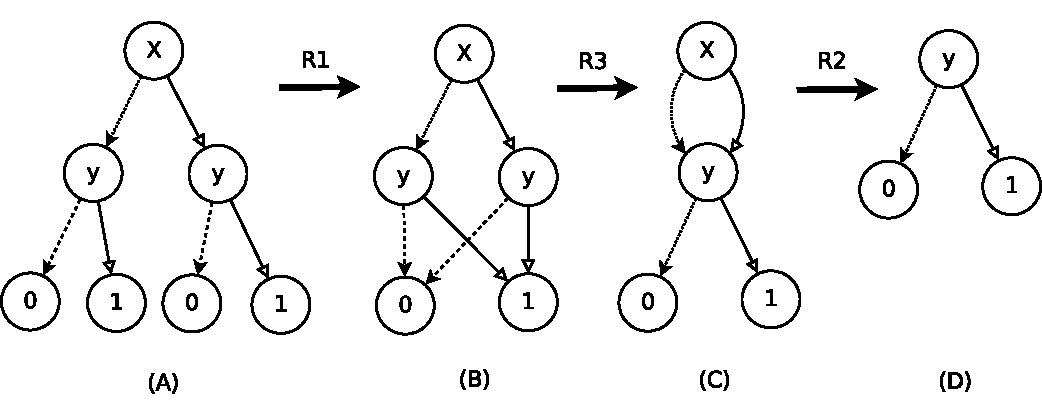
\includegraphics[scale=0.75]{Imagenes/reduccionBDD.pdf}
  \caption{Reducci\'on de un BDD seg\'un reglas R1,R2 y R3}
  \label{reduccionBDD}
\end{figure}
~\\

Si bien se logra con estas reglas reducir en gran proporci\'on cierto conjunto de BDDs, otros BDDs no son tan susceptibles a ser reducidos de esta manera. Un efecto negativo visible en mucho de estos es la reutilizaci\'on en sus nodos de una misma variable booleana, lo cual implica revisar el valor de aquellas m\'as de una vez. Otro defecto surge de que diferentes BDDs pueden representar una misma funci\'on booleana, por lo cual comparar la equidad de las funciones booleanas representadas en BDDs requiere de mucho trabajo.\\

Todas estas complicaciones logran ser evitadas usando un subconjunto de BDDs llamados \textit{diagramas de decisi\'on binaria ordenados} (OBDD). Los OBDD imponen un orden sobre la aparici\'on de las variables en sus nodos, evitando de este modo los BDDs con m\'as de una aparici\'on de la misma variables. Podemos dar la siguiente definici\'on de un OBDD\cite{Huth}:\\

\textit{Sea $[x_1,x_2,...,x_n]$ una lista ordenada de variables sin duplicados y sea B un BDD cuyas variables pertenecen a la lista. Decimos que B tiene el ordenamiento $[x_1,x_2,...,x_n]$ si todas las variables en los nodos de B ocurren en la lista, y para cada ocurrencia de $x_i$ seguida de $x_j$ en cualquier camino sobre B, pasa que $i < j$. Decimos entonces que un OBDD es un BDD que posee un orden para alguna lista de variables.}\\

Notemos que como corolario de la definici\'on obtenemos que una variable no puede ocurrir m\'as de una vez en el OBDD. Estos diagramas poseen adem\'as la cualidad de que para cada funci\'on booleana y orden de variables existe un \'unico OBDD reducido que la representa. Osea que si $B_1$ y $B_2$ son dos OBDD reducidos con orden de variables compatible que representan a la funci\'on booleana f entonces $B_1$ y $B_2$ son id\'enticos. Esto lleva a que la comparaci\'on de equidad entre los mismos se reduzca a una simple comparaci\'on entre sus nodos.
Cuando no podemos seguir reduciendo un OBDD seg\'un las reglas R1, R2 y R3, decimos que est\'a en su forma can\'onica. Son de inter\'es especial las formas can\'onicas de la figura \ref{canonicos} debido a que nos permiten identificar las siguientes situaciones:
\begin{itemize}
\item \textbf{Validez de una funci\'on:} podemos verificar validez de una funci\'on booleana (verificar si la funci\'on siempre computa 1) de la siguiente manera: reducimos su OBDD a su forma can\'onica, si el resultado de la reducci\'on es $B_1$ entonces la funci\'on es v\'alida.
\item \textbf{Implicaci\'on:} podemos verificar si la funci\'on $f(x_1,x_2,...,x_n)$ implica la funci\'on $g(x_1,x_2,...,x_n)$ (es decir si f computa 1 entonces g tambi\'en) reduciendo el OBDD obtenido como $f \wedge \neg g$. Si el OBDD can\'onico es distinto de $B_0$ entonces la implicancia es verdadera.
\item \textbf{Satisfactibilidad:} podemos verificar satisfactibilidad de una funci\'on $f(x_1,x_2,...,x_n)$ (es decir si f computa 1 para alguna asignaci\'on de ceros y unos a sus variables) reduciendo su OBDD a forma can\'onica y verificando que \'esta no sea $B_0$
\end{itemize}

El orden de variables elegido toma vital importancia, ya que de \'el depende el tama\~no del OBDD. Existen algoritmos que logran un ordenamiento inteligente de las variables para mantener acotado el tama\~no de almacenamiento necesario para el OBDD. As\'i tambi\'en existen algoritmos que hacen eficiente la reducci\'on de OBDDs a su OBDD can\'onico, como tambi\'en algoritmos que permiten computar conjunci\'on, disyunci\'on y negaci\'on de OBDDs con considerable eficiencia.\\


\begin{figure}
  \centering
    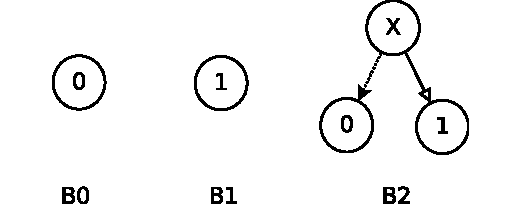
\includegraphics{Imagenes/canonicos.pdf}
  \caption{OBDDs can\'onicos de relevancia}
  \label{canonicos}
\end{figure}
~\\


El uso de BDDs produjo un gran salto en el model checking llevando en principios de los noventa a lograr verificar sistemas con espacios de estados mucho m\'as grandes que con m\'etodos anteriores. El model checking usando OBDDs es llamado \textbf{Model Checking Simb\'olico} y debe su nombre a que sugiere no representar cada estado por separado, sino que se representa en los OBDDs conjuntos de estados de manera simb\'olica, m\'as precisamente a aquellos estados que cumplen con la propiedad que esta siendo verificada.Veamos ahora como representar estos conjuntos de estados en OBDDs y como representar la relaci\'on de transici\'on entre ellos:

Recordemos que en nuestro modelo de sistema como estructura de Kripke hab\'iamos definido un conjunto de proposiciones at\'omicas sobre las variables del sistema, que represent\'abamos a cada estado como una valuaci\'on sobre las variables del sistema, y que la funci\'on de etiquetado L nos proporcionaba el subconjunto de AP que era v\'alido en cada estado. Tomaremos la primicia de que poseemos un orden sobre las proposiciones en AP dado como $(x_1,x_2,...,x_n)$ y representaremos ahora cada estado $s$ como un vector $(v_1,v_2,...,v_3)$ donde cada $v_i \in {0,1}$ y $v_i = 1$ si y solo si $x_i \in L(s)$. Vemos entonces que los estados son representados por la funci\'on caracter\'istica inducida por $L$. Es decir, la funci\'on booleana que representa un estado es aquella que valuada en $(v_1,v_2,...,v_3)$ computa el valor 1, y para cualquier otro valuaci\'on de sus variables computa el valor 0. En t\'erminos de OBDDs, el OBDD que representa al estado s es aquel que representa la funci\'on booleana : $$l_1 \wedge l_2 \wedge ... \wedge l_n$$ donde $l_i$ es $x_i$ si $x_i \in L(s)$ y $\neg x_i$ de lo contrario. Luego para un conjunto de estados $S = {s_1, s_2, ..., s_m}$ la representaci\'on en OBDD esta dada por aquel que representa a la funci\'on booleana $$(l_{11} \wedge l_{12} \wedge ... \wedge l_{1n}) \vee (l_{21} \wedge l_{22} \wedge ... \wedge l_{2n}) \vee ... \vee (l_{m1} \wedge l_{m2} \wedge ... \wedge l_{mn})$$ donde $(l_{i1} \wedge l_{i2} \wedge ... \wedge l_{in})$ representa al estado $x_i$.\\

Para el caso de la relaci\'on de transici\'on recordemos que \'esta es un subconjunto sobre $S\times S$. De nuevo podemos inducir la funci\'on booleana representante a partir de la funci\'on de etiquetado $L$. De este modo una relaci\'on $s\rightarrow s'$ en $R$ es representada por los vectores $(v_1,v_2,...,v_n),(v'_1,v'_2,...,v'_n)$, donde $v_i = 1$ si $p_i \in L(s)$ y 0 de lo contrario, y $v'_i = 1$ si $p_i \in L(s')$ y 0 de lo contrario. En t\'erminos de OBDD, representamos la relaci\'on con el OBDD para la funci\'on booleana $$(l_1,l_2,...,l_n) \wedge (l'_1,l'_2,...,l'_n)$$ y el conjunto representando el total de la relaci\'on $R$ se logra a partir de la conjunci\'on de cada una de estas f\'ormulas.








%TODO ver qu\'e hizo Pablo Dal Lago con esto, para ampliar la teor\'ia de reducci\'on.

%..................................................................................................................................................................





\section{L\'ogicas temporales}
Las l\'ogicas temporales son sistemas de reglas y s\'imbolos que nos permiten describir y razonar sobre proposiciones en t\'erminos del tiempo. En el caso del model checking, son de gran utilidad para la especificaci\'on de las propiedades a verificar sobre el modelo del sistema. A continuaci\'on presentaremos dos l\'ogicas temporales de inter\'es para este trabajo. Ambas l\'ogicas difieren en expresividad, por lo que hacer uso de las dos nos permite una mayor versatilidad al momento de especificar las propiedades deseadas.\\

\subsection{LTL}
La \textbf{L\'ogica de Tiempo Lineal (LTL)} nos permite razonar sobre ejecuciones lineales a trav\'es del tiempo. En cada instante de tiempo solo existe una \'unica ejecuci\'on real a realizarse. Com\'unmente esta ejecuci\'on de la que hablamos comienza en este momento y se extiende al infinito. El tiempo es discreto y podemos realizar un paralelismo entre el salto de un momento al otro y cada paso en la ejecuci\'on del sistema que se analice. As\'i, cada momento representa una configuraci\'on en el estado del sistema y cada salto en el tiempo representa una transici\'on desde un estado del sistema a uno nuevo. Estas l\'ogicas est\'an compuestas por un conjunto finito de proposiciones at\'omicas AP, los conectivos booleanos $\neg$, $\wedge$, $\vee$, $\rightarrow$, $\leftrightarrow$ y los conectivos temporales G, F, X, U, R. Estos \'ultimos conectivos se corresponden con las palabras en idioma ingl\'es \textbf{G}lobally, \textbf{F}inally, Ne\textbf{X}t, \textbf{U}ntil y \textbf{R}elease.\\ A continuaci\'on damos una descripci\'on intuitiva del significado de cada conectivo:
\begin{itemize}
\item G $\phi$ expresa que en todo momento vale $\phi$.
\item F $\phi$ expresa que $\phi$ se cumple en elg\'un momento.
\item X $\phi$ expresa que $\phi$ se cumple en el momento inmediatamente posterior al actual.
\item $\phi$ U $\psi$ expresa que $\psi$ vale en alg\'un momento, y para todo momento anterior a aquel $\phi$ vale.
\item $\phi$ R $\psi$ expresa que o bien $\phi$ no vale nunca y $\psi$ vale siempre, o bien $\psi$ vale en cada momento hasta que $\phi$ valga.
\end{itemize}
Usando LTL podemos expresar propiedades de \textit{safety} y \textit{liveness} de nuestro sistema de manera sencilla. Por ejemplo para expresar \textit{En alg\'un momento algo bueno suceder\'a} usamos  \textbf{F} 'algoBueno', o para expresar \textit{En ning\'un momento algo malo sucede} usar\'iamos \textbf{G} $\neg$ 'algoMalo'.\\

Es com\'un interpretar las f\'ormulas LTL sobre estructuras de Kripke. Una f\'ormula LTL puede ser satisfecha por una serie infinita de valuaciones sobre AP. Podemos ver a esta serie infinita como una palabra sobre una ejecuci\'on sobre una estructura de Kripke. De este modo si queremos saber si la formula $\phi$ se satisface en un sistema representado por la estructura de Kripke M, basta con ver que el lenguaje de M (todas las palabras posibles en M) satisfagan $\phi$. Definimos la sem\'antica de formulas LTL como sigue:\\

Sea la palabra $\omega$ = $s_1s_2s_3...$ de valuaciones en AP. Definimos la relaci\'on de satisfactibilidad $\models$ de una formula LTL con respecto a la palabra $\omega$ a partir de las siguientes reglas:
\begin{itemize}
\item $\omega \models p $ si $ p \in \omega[0]$
\item $\omega \models \neg p $ si no $\omega \models p$
\item $\omega \models \phi \vee \psi$ si $\omega \models \phi$ or $\omega \models \psi$
\item $\omega \models$ X $\phi$ si $\omega$[1...] $\models \phi$
\item $\omega \models \phi U \psi$ si existe $i \geq 0$ tal que  $\omega[i...] \models \psi$ y para todo $0 \leq k < i$, $\omega[k...] \models \phi$ 
\end{itemize}
Notar que los dem\'as conectivos son derivados de aquellos para los que hemos definido las reglas de satisfactibilidad. \\

Muchas veces es de inter\'es en model checking definir propiedades bajo \textbf{condiciones de equidad}, tambi\'en llamadas \textit{condiciones de \textbf{fairness}}. Por ejemplo en el contexto del modelado de un planificador de tareas podemos requerir que el mismo atienda equitativamente a los diferentes procesos. LTL a diferencia de CTL nos da la posibilidad de definir estas equidades:
\begin{enumerate}
\item Equidad incondicional: G F p (siempre finalmente se cumple p, o a menudo se cumple p)
\item Equidad fuerte: G F q $\rightarrow$ G F p (si a menudo vale q entonces a menudo vale p)
\item Equidad d\'ebil: F G q $\rightarrow$ G F p (si finalmente siempre vale q, entonces a menudo vale p)
\end{enumerate}


\subsection{CTL}
A diferencia de LTL, en la \textbf{L\'ogica de \'Arbol Computacional (CTL)} no existe en cada momento un \'unico camino a seguir. CTL es una l\'ogica de tiempo ramificado, en cada momento consideramos todos los posibles saltos hacia un estado posterior, y por lo tanto consideramos diferentes ejecuciones como posibles a realizarse en el futuro. Adem\'as de los conectivos l\'ogicos y temporales introducidos en LTL, CTL implementa el uso de los cuantificadores \textbf{A} (para todo camino) y \textbf{E} (existe un camino). A su vez establece la regla de estar obligado a usar estos cuantificadores delante de cada conectivo temporal, definiendo as\'i f\'ormulas sobre estados y no sobre caminos como lo hacen la l\'ogica LTL. CTL, a diferencia de LTL, nos permite hablar sobre la existencia de al menos un camino. As\'i es que podemos especificar propiedades como  \textit{E X p} y \textit{AG EF p}, las cuales no pueden ser especificadas en LTL ya que en ella no podemos hablar de la existencia de al menos un camino en el futuro en el cual se cumple 'p'.

Los conectivos ${\neg,\wedge,AX,AU,EU}$ comprenden un conjunto completo de conectivos para la l\'ogica CTL dado que los dem\'as pueden ser derivados a partir de ellos. Podemos decir que el siguiente es el significado intuitivo de estos conectivos:
\begin{itemize}
\item $\neg$ es la negaci\'on booleana usual.
\item $\wedge$ es la conjunci\'on booleana usual.
\item $AX~q$ se cumple en un estado $s$ si para cualquier ejecuci\'on, $q$ vale en el estado que sucede a $s$.
\item $EX~q$ se cumple en un estado $s$ si existe al menos una ejecuci\'on donde $q$ vale en el estado que sucede a $s$.
\item $E[p~U~q]$ se cumple en un estado $s$ si existe al menos una ejecuci\'on $s_1s_2...s_n...$ con $s_1 = s$ donde $q$ vale en $s_n$ y $p$ vale para todo estado en $s_1...s_{n-1}$.
\end{itemize}

A continuaci\'on, utilizando estructuras de Kripke, definimos la sem\'antica formal de CTL por inducci\'on estructural sobre una f\'ormula $\phi$. Sea la estructura de Kripke $M =(S,S_0,R,L)$ sobre AP, sea $\phi$ una f\'ormula CTL bien formada sobre AP, y sean s $\in$ S y p $\in$ AP.\\

\begin{tabularx}{\textwidth}{@{\textbullet}lcX}
$~M,s \models p$ & $\leftrightarrow$ & $p \in L(s)$\\
$~M,s \models \neg\phi $ & $\leftrightarrow$ & $ \text{no } M,s \models \phi$\\
$~M,s \models \phi_0 \wedge \phi_1 $ & $\leftrightarrow$ & $ M,s \models \phi_0 \text{ y } M,s \models \phi_1$\\
$~M,s \models AX\phi $ & $\leftrightarrow$ & $ \forall (s,s') \in R,~ M,s' \models \phi$\\
$~M,s \models EX\phi $ & $\leftrightarrow$ & $ \exists (s,s') \in R,~M \text{ tal que } s' \models \phi$\\
$~M,s \models E(\phi_0 U \phi_1) $ & $\leftrightarrow$ & $\exists \text{ una ejecuci\'on } s_1s_2s_3...s_n... \text{ definida por } R \text{ tal que }\linebreak  s_0 = s, M,s_n \models \phi_1, \forall 0<i<n~ M, s_i \models \phi_0$\\
\end{tabularx}




%..................................................................................................................................................................




\section{Caracter\'isticas del Model Checking}
Existen diferentes m\'etodos para la verificaci\'on de sistemas complejos, entre ellos podemos destacar como principales la simulaci\'on, el testing, la verificaci\'on deductiva, y el model checking\cite{Clarke}. Tanto la simulaci\'on como el testing comprenden realizar experimentos antes de desplegar el sistema en el campo. Mientras que en el caso de la \textit{simulaci\'on} se trabaja sobre una abstracci\'on o modelo del sistema, en el \textit{testing} se trabaja sobre el [producto real]. En cuanto a costo-eficiencia, estos m\'etodos pueden ser ventajosos para detectar gran cantidad de errores. Sin embargo, revisar todas las posibles interacciones y potenciales errores usando simulaci\'on y testing es raramente posible.\\
El t\'ermino \textit{verificaci\'on deductiva} normalmente refiere al uso de axiomas y reglas para probar la correctitud del sistema. Este m\'etodo si bien posee la ventaja de poder probar correctitud sobre sistemas de estados infinitos no es muy utilizado fuera de casos cr\'iticos. Esto se debe a que requiere de gran cantidad de tiempo y de la conducci\'on por parte de expertos en el campo del razonamiento l\'ogico.\\

\textbf{Model checking} es un m\'etodo autom\'atico para la verificaci\'on de propiedades sobres sistemas concurrentes finitos. Trabaja sobre un modelo del sistema y explora exhaustivamente todos sus posibles estados con el fin de verificar si una propiedad especificada sobre el mismo es verdadera o no. Presenta ciertas ventajas sobre los m\'etodos anteriormente mencionados:

\begin{itemize}
\item Detecta errores en etapas tempranas de dise\~no, evitando tener que replantear todo al encontrar estos errores en etapas posteriores.

\item Gran parte de su proceso es autom\'atico, por lo cual no requiere de personal experto en campos de la matem\'atica para llevar a cabo las tareas de verificaci\'on.

\item Es exhaustivo con respecto al conjunto de estados del sistema.

\item Ofrece clara evidencia del problema en el caso de encontrar que la propiedad deseada sobre el sistema no se cumpla.
\end{itemize}

Sin embargo model checking sufre del problema de explsi\'on de estados. Esto implica que f\'acilmente se llegue a sistemas en los que la cantidad de estados es tan grande que supera los l\'imites de memoria f\'isica del hardware sobre el que corre el programa de model checking. Muchos algoritmos y optimizaciones sobre los model checkers han ayudado a combatir este efecto, pero sin embargo el mismo persiste. Otra soluci\'on a este problema es llevar el modelado a una mayor abstracci\'on con el fin de disminuir la cantidad de estados finales. Al hacer esto debemos tomar en cuenta que la abstracci\'on debe preservar la no satisfactibilidad de las propiedades a verificar, en el caso que esta exista. Como vemos este proceso de abstracci\'on y refinamiento requiere muchas veces de personal experto, y es una de las barreras a superar si se desea lograr que el model checking se convierta enteramente en una herramienta \text{``push-button''}.\\

Christel Baier y Joost-Pieter Katoen en su libro "Principles of model checking" \cite{Baier} identifican las siguientes tareas como pasos para realizar el \textit{proceso de model checking} sobre el dise\~no de un sistema:

\begin{enumerate}
\item Fase de modelado:
\begin{itemize}
\item Modelar el sistema en consideraci\'on usando el lenguaje del model checker que se tenga a mano.
\item Realizar algunas simulaciones sobre el modelo como primera revisi\'on y r\'apida aceptaci\'on del mismo.
\item Describir las propiedades a verificar sobre el modelo usando el lenguaje espec\'ifico para esta tarea.
\end{itemize}
\item Fase de ejecuci\'on:\\\\
Ejecutar el model cheker para verificar la validez de una propiedad sobre el sistema modelado. 
\item Fase de an\'alisis:
\begin{itemize}
\item Si la propiedad result\'o ser v\'alida $\longrightarrow$ en el caso de haber m\'as propiedades a verificar, proceder con la verificaci\'on de las mismas.
\item Si la pripiedad fu\'e refutada $\longrightarrow$
\begin{enumerate}
\item analizar, a partir de simulaci\'on, el contraejemplo generado.
\item refinar el modelo, dise\~no o propiedad.
\item repetir todo el proceso.
\end{enumerate}
\item La computadora se qued\'o sin memoria $\longrightarrow$ intentar reducir el modelo y empezar de nuevo.
\end{itemize}
\end{enumerate}


\begin{figure}[H]
  \centering
    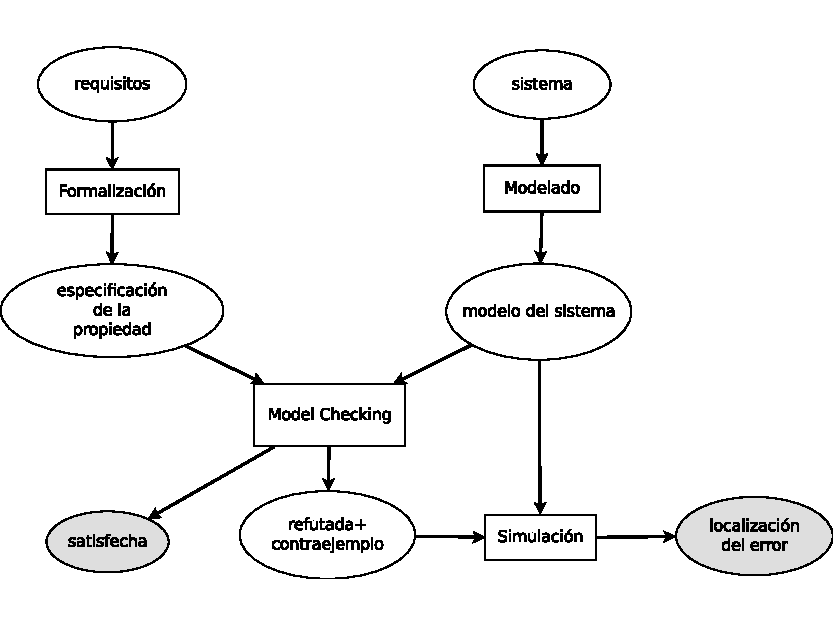
\includegraphics{Imagenes/procesoMC4.pdf}
  \caption{El proceso de Model Checking}
  \label{ltsakripke}
\end{figure}
~\\


En la fase de modelado podemos distinguir entonces por un lado el modelado del sistema y por otro la especificaci\'on de las propiedades. El modelado del sistema si bien algunas veces suele ser una simple compilaci\'on al lenguaje de modelado espec\'ifico de la herramienta de model checkin, otras veces puede requerir depuraci\'on del modelo para eliminar caracter\'isticas innecesarias que puedan ocasionar una explosi\'on de estados a tal grado de agotarse la memoria. Por otro lado podemos destacar como asunto importante en la etapa de especificaci\'on de propiedades el hecho de lograr completitud sobre las caracter\'isticas deseadas del sistema. Es decir que es esencial en esta etapa lograr expresar en las propiedades el conjunto completo de caracter\'isticas que se desea que el sistema posea.\\

La fase de ejecuci\'on usualmente es autom\'atica y solo consta de proveer al model checker con el modelado del sistema y la especificaci\'on de una propiedad para que el mismo decida sobre su validez.\\

Por \'ultimo, es en la fase de an\'alisis donde podemos decidir ya sobre el resultado de la verificaci\'on. Se pueden presentar varios escenarios: por un lado puede que el proceso de verificaci\'on no se haya completado debido al agotamiento de memoria, en tal caso se deber\'a recurrir al refinamiento del sistema para conseguir disminuir la explosi\'on de estados, o bien se deber\'a usar un equipo de mayor potencial en el caso de que ya no se logre llegar a un refinamiento significativo. Puede ser el caso de que todas las propiedades hayan sido validadas por el model checker, lo que indicar\'ia que el modelo del sistema cumple con las caracter\'isticas expresadas en la especificaci\'on de las propiedades. Por \'ultimo puede suceder que una o m\'as propiedades hayan sido refutadas. En este usualmente un contraejemplo otorgado por la herramienta nos permite identificar el problema, el cual puede haber sido causado por una mal modelado del sistema, una falla en la especificaci\'on, o simplemente porque en efecto el sistema no cumple con la caracter\'istica deseada.\\

Es importante tomar en cuenta que el \'exito de la verificaci\'on depende fuertemente de la correctitud en el modelado del sistema y la especificaci\'on de las propiedades. El sistema puede tener errores pero haber sido modelado evitando los mismos, lo cual puede llevar a que el model checker entregue falsos positivos. Este efecto tambi\'en puede ser causa de una especificaci\'on incompleta o err\'onea de las caracter\'isticas a verificar.\\




%%%%%%%%%%%%%%%%%%%%%%%%%%%%%%%%%%%%%%%%%%%%%%%%%%%%%%%%%%%%%%%%%%%%%%%%%%%%%%%%%%%%%%%%%%%%%%%%%%%%%%%%%%%%%%%%%%%%%%%%%%%%%%%%%%%%%%%%%%%%%%%%%%%%%%%%%%%%%%%%%%



\chapter{NuSMV}
\section{El model checker NuSMV}

NuSMV es un model chcker simb\'olico originado en la reingenier\'ia, reimplementaci\'on y extensi\'on de SMV, el primer model checker basado en BDD. NuSMV fue dise\~nado para ser una plataforma bien estructurada, de c\'odigo abierto, flexible, y ampliamente documentada, para el model checking. Con el fin de permitir que NuSMV sea utilizado en proyectos para la transferencia de tecnolog\'ias, fue dise\~nado para ser muy robusto, cercano a los est\'andares industriales, y para permitir lenguajes de especificaci\'on ampliamente expresivos\cite{Cimatti}.\\

NuSMV nos permite la verificaci\'on de propiedades en los formalismos LTL y CTL, sobre la especificaci\'on de sistemas finitos [s\'incronos y as\'incronos], bajo condiciones de fairness.\\

\textit{NuSMV2}, el cual es utilizado en este trabajo, integra la verificaci\'on en base a \textit{BDD} junto con la verificaci\'on acotada de propiedades LTL mediante \textit{SAT-Solving}. Otra particularidad de esta versi\'on es el uso de una licencia \textit{OpenSource} para programaci\'on y distribuci\'on abierta de su c\'odigo, lo cual permite, a cualquier persona interesada, usar la herramienta gratuitamente y colaborar con el desarrollo de la misma.


\section{Lenguaje de modelado de NuSMV}
Si bien el lenguaje de modelado de NuSMV es amplio y nos presenta diferentes posibilidades para la definici\'on de la maquina de estados, presentaremos en esta secci\'on solo aquella porci\'on que nos servir\'a m\'as adelante para compilar los modelos descriptos en el lenguaje de Falluto 2.0.\\

Cada proceso del sistema se describe en NuSMV como un m\'odulo, introducido por la palabra \textbf{MODULE}. Al menos uno de estos m\'odulos debe llamarse \textit{main}, y ser\'a el primero en ser [...]. Podemos ver cada proceso como una maquina de estados independiente y al conjunto de estos y sus interacciones como la maquina de estados que representa al sistema completo. Veamos entonces como definir la maquina de estado de cada proceso:\\

\textit{VARIABLES}\\

Dentro de cada \textit{m\'odulo}, introduciendo la secci\'on de variables por la palabra \textbf{VAR}, definimos las variables del proceso junto con sus dominios. Poseemos tres tipos b\'asicos de variables, las booleanas, las enteras y las enumeradas. Tenemos la posibilidad de declarar una variable como un arreglo de valores de cualquiera de los tipos anteriormente mencionados. Vemos un ejemplo a continuaci\'on:
\begin{verbatim}
MODULE main
    VAR
        var1 : boolean;
        var2 : -2..3;
        var3 : {a1, something, 42};
        var4 : array -1..2 of boolean;
\end{verbatim}
Vemos que en el ejemplo la variable \textit{var1} es de tipo booleano (su dominio est\'a formado por los valores \textit{TRUE} y \textit{FALSE}) , \textit{var2} es de tipo entero y su dominio se extiende desde el numero -2 al 3 y \textit{var3} es de tipo enumerado y su dominio lo forman las 3 palabras encerradas en llaves. Por \'ultimo \textit{var4} es un vector de 4 booleanos indexado desde el -1 al 2. Recordemos que las valuaciones sobre las variables representan el estado del proceso y una valuaci\'on sobre el conjunto de todas las variables de cada proceso representa el estado del sistema completo.\\

\textit{ESTADO INICIAL}\\

Para definir el conjunto de estados inicial de cada proceso introducimos una nueva secci\'on dentro del m\'odulo usando la palabra clave \textbf{INIT}, y hacemos uso de una f\'ormula proposicional sobre las variables del m\'odulo para restringir el subconjunto de estados que deseamos sea el inicial. Recordemos que seg\'un lo visto en la secci\'on \ref{} para cualquier conjunto de estados podemos definir una f\'ormula tal que solo ellos la cumplan.
\begin{verbatim}
MODULE auto
    VAR
        estado: {encendido, apagado}
        nafta: 0..3
    INIT
        estado = apagado & nafta = 3
\end{verbatim}
~\\

\textit{TRANSICIONES}\\

La palabra clave \textbf{TRANS} en NuSMV nos permite introducir dentro de los m\'odulos una secci\'on donde definir las transiciones de nuestra maquina de estados. As\'i como ya hemos planteado anteriormente, las transiciones hablar\'an sobre dos clases de estados: los estados actuales, y los estados posteriores, de manera de definir la relaci\'on sobre los mismos. Dada una variable de estado \textit{x}, tenemos que \textit{next(x)} representa el estado de la variables en el momento inmediatamente posterior al actual. Una formula proposicional establece entonces las caracter\'isticas de la relaci\'on de transici\'on. Las ambigüedades en esta f\'ormula con respecto a la maquina de estados representada introducen una elecci\'on aleatoria por parte de NuSMV. Esto es \'util para representar no determinismo entre saltos de estados.

\begin{verbatim}
MODULE auto
    VAR
        estado: {encendido, apagado}
        nafta: 0..3
    INIT
        estado = apagado & nafta = 3

    TRANS
        ( estado = encendido & nafta <= 0 ) -> ( next(estado) = apagado )

\end{verbatim}

Notemos que en el ejemplo solo definimos condiciones para el caso en que $estado = encendido$ y $nafta <= 0$, caso en el que el auto deber\'ia apagarse en el pr\'oximo estado. En los casos en que se da $estado = apagado$ o $nafta > 0$ el no-determinismo maneja la elecci\'on de un estado posterior.\\\\


\textit{RESTRICCIONES Y FAIRNESS}\\

NuSMV nos permite establecer restricciones de fairness sobre la ejecuci\'on de nuestro sistema. Esto nos permite revisar nuestro sistema bajo ciertos supuestos con respecto a su ejecuci\'on. Tenemos la posibilidad de definir dos tipos de condiciones de fairness sobre nuestro sistema modelado:
\begin{itemize}

\item \textbf{Fairness incondicional} Dada una f\'ormula \textit{q} sobre el estado del sistema, escribimos \textit{FAIRNESS q} para establecer una la condici\'on de fairness incondicional sobre nuestro sistema modelado. Establece que cierta condici\'on \textit{q} se cumple frecuentemente durante la ejecuci\'on del sistema. En t\'erminos de l\'ogicas de tiempo lineal, esto corresponder\'ia a restringir la ejecuci\'on del sistema a solo aquellas trazas donde se cumpla \textit{G F q}.

\item \textbf{Strong Fairness} Dadas dos f\'ormulas \textit{p} y \textit{q} sobre el estado del sistema, escribimos \textit{COMPASSION(p,q)} para establecer una condici\'on de fairness fuerte sobre el sistema. Esta condici\'on restringe a la revisi\'on de aquellas ejecuciones del sistema en donde valga que si \textit{p} se cumple siempre a menudo entonces \textit{q} se cumple siempre a menudo. En t\'erminos de LTL esto corresponder\'ia a revisar solo aquellas ejecuciones donde se cumpla \textit{G F p $\rightarrow$ G F q}.

\end{itemize}

~\\
\textit{PROPIEDADES Y VERIFICACI\'oN}\\

NuSMV nos permite verificar tanto propiedades LTL como CTL sobre nuestro sistema. Para cada una de ellas tenemos su respectiva palabra clave y la precedemos con la f\'ormula que exprese la propiedad a verificar. La verificaci\'on de estas propiedades se realizara bajo las condiciones que establecen las restricciones de fairness definidas. A continuaci\'on mostramos un ejemplo que ilustra la especificaci\'on de las propiedades:

\begin{verbatim}
MODULE auto
    VAR
        estado: {encendido, apagado}
        nafta: 0..3
    INIT
        estado = apagado & nafta = 3

    TRANS
        ( estado = encendido & nafta <= 0 ) -> ( next(estado) = apagado )


FAIRNESS nafta > 0

LTLSPEC F nafta = 0

CTLSPEC EG estado = apagado

\end{verbatim}



%%%%%%%%%%%%%%%%%%%%%%%%%%%%%%%%%%%%%%%%%%%%%%%%%%%%%%%%%%%%%%%%%%%%%%%%%%%%%%%%%%%%%%%%%%%%%%%%%%%%%%%%%%%%%%%%%%%%%%%%%%%%%%%%%%%%%%%%%%%%%%%%%%%%%%%%%%%%%%%%%%


\chapter{La sintaxis de Falluto2.0}

En este cap\'itulo repasaremos de manera detallada la sintaxis de Falluto2.0. Comenzaremos explicando como modelar el comportamiento operacional de nuestro sistema. A continuaci\'on mostraremos el mecanismo para la inyecci\'on de fallas sobre este sistema, y concluiremos describiendo la sintaxis para la especificaci\'on de restricciones y propiedades a verificar sobre el sistema. Para una referencia a\'un m\'as completa y precisa sobre las reglas sint\'acticas, en el ap\'endice \ref{} de este mismo trabajo se puede encontrar una descripci\'on de la sintaxis en t\'erminos de Parsing Expresion Grammars. Podemos encontrar ejemplos esclarecedores también en ref{}.

\section{Lenguaje de modelado de comportamiento operacional}
Para definir el comportamiento de cada proceso involucrado en el funcionamiento de nuestro sistema, usaremos los \textit{Proctypes} de Falluto2.0. Cada \textit{proctype} comprende en su totalidad el funcionamiento de una clase de proceso, y los procesos reales pueden ser instanciados a partir del mismo. La declaraci\'on de un \textit{proctype} es introducida mediante la palabra clave \textit{PROCTYPE}. A continuaci\'on se establece un nombre para esta clase de procesos, y se especifica si poseer\'a o no variables de contexto, y acciones de sincronizaci\'on. Podemos decir que todo esto forma parte del encabezado del \textit{proctype}:
\begin{verbatim}
PROCTYPE miProceso ( ctxVar1, ctxVar2 ; sinchroAct1, sinchroAct2 )
\end{verbatim}
En el cuerpo del \textit{proctype} podemos distinguir tres secciones que definen su comportamiento operacional. Las describimos a continuaci\'on:
\begin{enumerate}
\item \textbf{Declaraci\'on de variables de estado.} Introducido por la palabra clave \textit{VAR}, esta secci\'on se utiliza para declarar las variables que representan el estado del proceso. Semejante a la sintaxis de NuSMV, podemos declarar tres tipos de variables, sumado a la posibilidad de poder declarar vectores de variables de un tipo determinado. Podemos entonces declarar variables de tipo:
\begin{enumerate}
\item \textbf{Booleano.} Corresponden a aquellas variables que solo toman los valores TRUE y FALSE. Las declaramos con la siguiente sintaxis: \begin{verbatim}nombre_de_variable : bool\end{verbatim}
\item \textbf{Entero.} A las variables de tipo entero las declaramos d\'andoles un nombre y acompañ\'andolas con la especificaci\'on del rango entero sobre el cual pueden tomar valor. Por ejemplo una variable declarada como sigue, solo podr\'a tomar valores enteros entre -5 y 7: \begin{verbatim}nombre_de_variable : -5..7\end{verbatim}
\item \textbf{Enumerado.} Corresponden a las variables de tipo enumerado. Los valores que toman estas variables son definidos como un conjunto de palabras elegidas por el usuario. La sintaxis declarativa de este tipo de variables se asemeja al ejemplo que sigue: \begin{verbatim}nombre_de_variable : {a, casa, 34, a2}\end{verbatim}
\item \textbf{Vector.} Podemos declarar variables de tipo vector, eligiendo alguno de los anteriores como subtipo. El subtipo es el tipo de cada valor perteneciente al vector. De este modo podemos declarar vectores de booleanos, o vectores de enteros o de tipo enumerado. Se [contribuye] a la declaraci\'on de los vectores con un rango indicando la indexaci\'on del vector. El ejemplo que sigue es un vector de subtipo enumerado, y se indexa desde el -1 al 2: \begin{verbatim}nombre_de_variable : array -1..2 of {a,b,c}\end{verbatim}
\end{enumerate}
\item \textbf{Declaraci\'on de estados iniciales.}
Esta secci\'on es introducida por la palabra clave \textit{INIT}, y define el conjunto de estados iniciales de los procesos de este tipo mediante una formula proposicional sobre las variables de estado del proceso. Similar a la secci\'on INIT de los m\'odulos de NuSMV, la f\'ormula que se describe aqu\'i busca restringir o no los valores que puede adoptar cada variables de estado en el estado inicial de la ejecuci\'on del proceso. Se permite aqu\'i el uso de conectivos l\'ogicos y proposicionales como $\rightarrow, |, \&, \leftrightarrow, etc$, adem\'as de conectivos matem\'aticos, valores booleanos y otros elementos. La restricci\'on mas importante es que la f\'ormula final sea de tipo booleano.
\item \textbf{Definici\'on de las transiciones.}
Para definir la relaci\'on de transici\'on de nuestros procesos, tomaremos en cuenta cada transici\'on por separado. Podremos etiquetar las transiciones con un nombre. y de esta manera podernos referir a la misma en el momento de la verificaci\'on. Llamaremos acci\'on al nombre de la transici\'on. La sintaxis general para la declaraci\'on de una transici\'on es la que sigue: \begin{verbatim}[accion] condici\'on_de_habilitaci\'on => postcondici\'on ;\end{verbatim}
Como ya dijimos \textit{accion} es el nombre de la transici\'on (representa a la acci\'on que lleva a cabo el sistema para pasar a un nuevo estado), la \textit{condici\'on de habilitaci\'on} es una f\'ormula booleana sobre el estado actual del sistema, que restringe los estados de partida de la transici\'on a aquellos que la cumplan. La postcondici\'on es un lista de asignaciones a las variables en el estado de llegada. Estas asignaciones definen las caracter\'isticas de los estados de destino de esta acci\'on. Para indicar que estamos asignando un valor a una variable en el pr\'oximo estado usamos el apostrofe al final del nombre de la variable, por ejemplo si $x$ es una variable en el estado actual entonces $x'$ es una variables en el estado inmediatamente pr\'oximo. El siguiente es un ejemplo un poco mas claro para la declaraci\'on de una transici\'on:\begin{verbatim}[transicion1] x > 3 & y => x' = x - 1, y' = !y;\end{verbatim}
\end{enumerate}

Una vez descripto el funcionamiento de los procesos dentro de cada proctype, podemos instanciar una o mas veces cada uno de ellos para en efecto definir los procesos involucrados en el sistema. Usamos para ello la palabra clave INSTANCE y pasamos a la instanciación los parámetros pertinentes, según se haya definido en el proctype correspondiente. La sintaxis sería entonces la siguiente: \begin{verbatim}INSTANCE nombre = nombre_proctype(parametro1, parametro2, ..., parametroN\end{verbatim}
Como ya hemos mencionado, podemos pasar variables de contexto como parámetros a nuestras instancias. Estas variables de contexto pueden ser referencias a instancias, o a variables de otras instancias. Para pasar una instancia completa como variable de contexto simplemente colocamos su nombre en el parámetro correspondiente. Para referir a una variable en particular de alguna instancia, usamos la construcción $nombre\_de\_instancia.nombre\_de\_variable$.\\

En cuanto a los parámetros de acciones de sincronización, basta con pasar un nombre a elección al parámetro. Todas las acciones con el mismo nombre a nivel de instanciación, serán sincronizadas entre si. Es decir que si quiero sincronizar acciones entre distintas instancias debo tener presente estas acciones parametrizadas en el proctype, y debo otorgarles un mismo nombre en la instanciación de los procesos involucrados.

\section{Lenguaje de descripci\'on de fallas}
En Falluto2.0 podemos inyectar f\'acilmente fallas en los procesos definidos. Las fallas forman parte de cada proceso y por lo tanto son declaradas dentro de los proctypes en una subsecci\'on introducida por la palabra clave \textit{FAULT}. La sintaxis general para la inyecci\'on de una falla es la siguiente: \begin{verbatim}nombre : condicion_habilitacion => postcondicion is tipo\end{verbatim}
Como vemos cada falla tiene un nombre, y su sintaxis es similar a la de una transici\'on com\'un. Esto se debe a que se toma en cuenta la falla como una transici\'on m\'as, aunque no deseada, del sistema. El nombre le otorga a la falla una identificaci\'on \'unica dentro del proctype. La condici\'on de habilitaci\'on es nuevamente una f\'ormula booleana sobre el estado actual del proceso (y el sistema global si tomamos en cuenta el uso de las variables de contexto). La postcondici\'on establece condiciones a cumplirse en el estado de llegada luego de la transici\'on de falla. De nuevo, se introduce aqu\'i una lista de asignaciones a las variables de estado a ser cumplidas por el estado de llegada. Las fallas pueden pertenecer a tres tipos en particular: \textit{transient, stop, byzantine}. Podemos distinguir dos clases de fallas seg\'un la prolongaci\'on de su actividad. Las fallas transient pertenecen a una clase de fallas en donde el efecto es instantaneo, mientras que las fallas de tipo stop y byzantine pertenecen a una clase de fallas de efecto permanente. A continuaci\'on daremos la sintaxis para declarar cada uno de estos tipos para las fallas:\\

\begin{itemize}
\item \textbf{Tipo Transient.} Simplemente usamos la palabra clave \textit{TRANSIENT} para declarar que la falla pertenece a este tipo. Notar que los efectos de estas fallas se restringen a la postcondici\'on que se haya definido en la declaraci\'on de la misma. Ejemplo: \begin{verbatim}falla1 : TRUE => x' = 0 is TRANSIENT\end{verbatim}
\item \textbf{Tipo Stop.} Declara que la falla tiene la capacidad de detener total o parcialmente el funcionamiento del proceso, impidiendo que el mismo realice ciertas transiciones. Usamos la palabra clave STOP y opcionalmente la precedemos de una lista con los nombres de transiciones que esta falla, en el caso de ocurrir, inhabilita. Notemos que si optamos por no otorgar dicha lista, la falla detendr\'a todas las transiciones normales del sistema, entendiendo por normales a aquellas que no son transici\'on de falla. Ejemplo: \begin{verbatim}falla1 : x => y' = FALSE is STOP(trans1,trans2) \end{verbatim}
\item \textbf{Tipo Byzantine.} Declara que la falla provoca un efecto bizantino sobre ciertas variables del proceso, es decir que una vez ocurrida la falla las variables mencionadas podr\'an en cualquier momento cambiar su valor actual por alg\'un otro valor dentro de su dominio, afectando as\'i el estado del sistema. Debemos preceder a la palabra clave BYZ con una lista de nombres de variables que ser\'an afectadas. Ejemplo: \begin{verbatim}falla1: TRUE => ... is BYZ(var1, var2) \end{verbatim}
\end{itemize}

\section{Lenguaje de especificación de propiedades y restricciones}

Con el fin de poder especificar propiedades a cerca de nuestro sistema para su posterior verificación, Falluto2.0 nos ofrece la posibilidad de trabajar sobre los lenguajes de especificación LTL y CTL. Se propone también el uso de meta-propiedades para razonar sobre el comportamiento del sistema bajo los efectos de fallas.
Para la especificación de una propiedad LTL usamos la palabra clave LTLSPEC y la precedemos de una fórmula LTL que defina la propiedad deseada sobre el total del sistema. Podemos usar para ello operadores LTL comunes como G (Globaly), F(Finaly), etc, además de los conectivos y operadores de la lógica proposicional. Similarmente para definir propiedades en lógica CTL usamos la palabra clave CTLSPEC precedida por la fórmula correspondiente. La sintaxis completa para la formación de las formulas puede encontrarse en el apéndice \ref{}.\\
Falluto2.0 posee además las siguientes meta-propiedades para la verificación del sistema:
\begin{itemize}
\item \textbf{Normal Behaiviour} Usamos esta propiedad para verificar propiedades bajo la premisa de que no ocurren fallas durante la ejecución del sistema. Usamos la palabra clave NORMAL\_BEHAVIOUR y la precedemos por una fórmula LTL o CTL especificando la propiedad deseada. Luego la propiedad será satisfecha por el sistema si el mismo la satisface en todas aquellas ejecuciones donde no ocurren fallas. La sintaxis es entonces: \begin{verbatim}NORMAL_BEHAVIOUR -> q \end{verbatim} donde $q$ es una fórmula expresada en LTL o CTL.
\item \textbf{Finitely Many Fault/s} Utilizando la sintaxis \begin{verbatim}FINITELY_MANY_FAULT(fault1, fault2, ..., faultn) -> q\end{verbatim} podemos verificar si la propiedad $q$ se cumple bajo la suposición de que eventualmente dejan de ocurrir las fallas de nombre $fault1$, $fault2$, ..., $faultn$ en la ejecución del sistema. En este caso la propiedad $q$ solo puede estar escrita en LTL debido a restricciones intrínsecas de la lógica CTL. De manera similar el uso de la construcción \begin{verbatim}FINITELY_MANY_FAULTS -> q \end{verbatim} permite verificar si la propiedad $q$ se cumple bajo la suposición de que finalmente deja de ocurrir falla alguna en el sistema, y el mismo pasa a transitar por transiciones normales.
\item \textbf{Deadlock check} La utilización de la palabra clave CHECK\_DEADLOCK dentro de la sección de opciones en la especificación de nuestro sistema, ordena la verificación de que nuestro sistema no caiga en deadlock. Es decir que con esta palabra clave podemos verificar si en algún momento el sistema se ve impedido a realizar transiciones normales, y debe optar por detenerse o realizar transiciones de falla.
\end{itemize}

Podemos restringir la verificación de las propiedades sobres nuestro sistema utilizando condiciones de fairness. Para ello poseemos las dos siguientes construcciones:
\begin{itemize}
\item \textbf{Fairness incondicional.} Para restringir la verificación del sistema a solo aquellas ejecuciones donde una propiedad $q$ se cumpla siempre a menudo, usamos la siguiente sintaxis: \begin{verbatim}FAIRNESS q\end{verbatim} donde $q$ es una fórmula proposicional que habla a cerca del estado del sistema.
\item \textbf{Fairnes fuerte.} Dadas dos formulas proposicionales $p$ y $q$ sobre nuestro sistema, podemos restringir la verificación de propiedades LTL a ejecuciones en las cuales se cumpla la condición de justicia fuerte de $p$ con respecto a $q$ usando la siguiente sintaxis: \begin{verbatim}COMPASSION(p,q)\end{verbatim} De esta manera restringimos la verificación solo a ejecuciones donde se cumpla que si $p$ vale siempre a menudo, entonces $q$ vale siempre a menudo. Tomemos en cuenta que el uso de esta construcción no es compatible con propiedades definidas en CTL y puede dar resultados erróneos.
\end{itemize}

%%%%%%%%%%%%%%%%%%%%%%%%%%%%%%%%%%%%%%%%%%%%%%%%%%%%%%%%%%%%%%%%%%%%%%%%%%%%%%%%%%%%%%%%%%%%%%%%%%%%%%%%%%%%%%%%%%%%%%%%%%%%%%%%%%%%%%%%%%%%%%%%%%%%%%%%%%%%%%%%%%


\chapter{Semántica de Falluto2.0}
Como ya mencionamos en la introducción a este trabajo, Falluto2.0 es un front-end para NuSMV. Por lo tanto la descripción del sistema en el lenguaje de Falluto2.0 debe ser compilada a una descripción en el lenguaje de NuSMV. Para ello es necesario tomar en cuenta la semántica de Falluto2.0. En este capítulo abordaremos el tema de la semántica de Falluto2.0, repasando las ideas detrás de su implementación y dando una mirada a la compilación al lenguaje de NuSMV.

\section{Construcción de un sistema global de procesos concurrentes}
En la estructura de la especificación del sistema en Falluto2.0 podemos distinguir la definición del comportamiento de los procesos, llevado a cabo a partir de los proctypes, de la instanciación de los diferentes procesos. Se busca que los procesos se desarrollen de manera concurrente en el entorno del sistema global, donde cada procesos pueda tener acceso a cierta información del sistema según lo defina el usuario. Se busca así también que los procesos puedan sincronizar acciones y que se pueda controlar de manera general el interliving del resto de las acciones.
La representación del sistema completo se logra en la compilación a partir del uso de un solo módulo de NuSMV con el siguiente aspecto:
\begin{verbatim}
MODULE main
VAR
...
INIT
...
TRANS
...
\end{verbatim}
A continuación describiremos como se rellena cada sección de este módulo con el fin de lograr la compilación del sistema original descripto usando el lenguaje de Falluto2.0.\\

\textbf{VARIABLES DEL SISTEMA}
Podemos ver el estado del sistema como aquel formado por la conjunción del estado de cada proceso que lo compone. De este modo las variables de estado del sistema compilado serán la unión de todas las variables de estado de cada instancia declarada en el sistema original. En la sección VAR entonces colocaremos por cada variables de cada instancia del sistema una variables en representación. La univocidad de las mismas estará dada por la univocidad del nombre de cada instancia con respecto a sus pares. Otras variables formarán parte de esta sección también:
\begin{itemize}
\item \textbf{Variable de acción} Esta variables nos permitirá denotar cual fue la última acción llevada a cabo por el sistema. Su utilidad sin embargo va mas allá de una simple denotación, ya que nos permitirá especificar sobre las acciones llevadas a cabo por el sistema. De esta manera podremos hablar sobre propiedades a cerca del accionar del mismo y establecer restricciones sobre el mismo. El dominio de esta variables entonces consta de palabras denotando la realización de cada acción del sistema, entre ellas las acciones comunes de cada instancia de proceso, las acciones de falla de cada instancia de proceso, y acciones de efectos de fallas bizantinas. Un último valor en el dominio de esta variable nos permite denotar una transición al estado de deadlock.
\item \textbf{Variables de activación de fallas} Las fallas permanentes, es decir las de tipo STOP y BYZANTINE, poseen una variable booleana que nos permite conocer si las estas fallas han ocurrido y están afectando el funcionamiento del sistema.
\item \textbf{Variables de program counter} Estas variables permiten distinguir entre las acciones de igual nombre dentro de un mismo proceso. Existe entonces un variable de este tipo por cada proceso instanciado. Nos permiten eliminar casos de ambigüedad en el salto de estados del sistema, que de otro modo nos llevaría a una representación errónea del sistema original.
\end{itemize}
~\\

\textbf{ESTADOS INICIALES}
Como ya dijimos, la restricción de estados iniciales en NuSMV se lleva a cabo a partir de una fórmula booleana dentro de la sección \textit{INIT} del módulo. Nuestra fórmula booleana será entonces la conjunción booleana de todas las formulas booleanas presentes en la sección \textit{INIT} de cada proceso instanciado. Agregaremos también en esta fórmula condiciones para la inicialización de variables introducidas por la compilación como serían las variables de actividad de falla y las de program counter.\\

\textbf{TRANSICIONES}
La relación de transición esta representada en la sección \textit{TRANS} del módulo compilado mediante una fórmula booleana que captura cuatro tipos de transiciones sin realizar distinción entre ellas. Nos aseguramos que estas transiciones sean excluyentes de manera de representar correctamente el modelo diseñado en el lenguaje de Falluto2.0. Esta exclusión se lleva a cabo a partir de la variable de acción introducida en el momento de compilación, y en el caso de no ser suficiente con ella, usamos también las variables de program counter (por ejemplo cuando hay mas de una acción con el mismo nombre dentro del mismo proctype). Los cuatro tipos de transiciones corresponden a:
\begin{itemize}
\item \textbf{Acciones comunes.} Son las transiciones definidas dentro de cada la sección TRANS de cada proctype.
\item \textbf{Acciones de falla.} Son las correspondiente a las transiciones de estados llevadas a cabo a partir de las fallas declaradas en la sección \textit{FAULT} de cada \textit{proctype}.
\item \textbf{Acciones de efecto bizantino.} Representan el cambio de estado del sistema como consecuencia del accionar de los efectos de una falla bizantina.
\item \textbf{Acción de deadlock.} Representa la imposibilidad de realizar cualquier acción normal. Decimos entonces que el sistema ha realizado una transición hacia un estado de deadlock. Veremos mas adelante la utilidad de poseer esta transición.
\end{itemize}
La disyunción excluyente de estas transiciones forma la fórmula de transición final que introducimos en la sección \textit{TRANS} de nuestro módulo compilado. Nuestro módulo de NuSMV quedará en términos de lo que sigue:
\begin{verbatim}
MODULE main
VAR
    * Por cada instancia de proceso, introducimos la lista 
      de variables declaradas en su respectivo proctype.
    * Variable de accion.
    * Variables de actividad de fallas permanentes.
    * Variables de program counter por cada proceso instanciado.
INIT
    Conjuncion de formulas de la seccion INIT de procesos instanciados
    & Inicializacion de variables introducidas en compilacion.
TRANS
    disyuncion de transiciones comunes compiladas 
    | disyuncion de transiciones de falla compiladas 
    | disyuncion de transiciones de efectos bizantinos 
    | transicion de deadlock
\end{verbatim}


\section{Compilación de transiciones}
Veremos a continuación como se realiza el proceso de compilación de cada una de las transiciones que luego forman parte de la formula de la sección \textit{TRANS} del módulo compilado.\\

\textbf{TRANSICIONES NORMALES}
Recordemos que la siguiente era la sintaxis general de la declaración de una transición NORMAL en el lenguaje de Falluto2.0 (Para mas detalles referirse al capítulo \ref{}):
$$[nombre]~habilitacion => postcondicion;$$
La versión compilada de esta acción tendrá el siguiente aspecto:
$$next(actvar)=nombre~\&~!faultact~\&~habilitacion~\&~postcondicion~\&~resto$$
Notar que de darse esta acción, el nombre de la misma quedará guardado como valor de actvar en el próximo estado, indicando que la acción que se llevo a cabo para llegar a ese estado fue en efecto esta. \textit{!faultact} es un fórmula que asegura que no estén activas aquellas fallas de tipo STOP que afectan esta transición. En efecto esta fórmula es simplemente la conjunción de la negación de las variables de actividad de falla para aquellas fallas que afectan esta transición. \textit{habilitacion} es simplemente una compilación directa de la fórmula de habilitación original al igual que \textit{postcondicion} la cual es la conjunción de la compilación directa de las asignaciones establecidas en la postcondición original. Por último en \textit{resto} nos aseguramos que en el próximo estado no cambie el valor de las variables cuyo valor no es definido en esta transición. En efecto esta fórmula es la conjunción de las asignaciones $next(x)=x$ por cada variable x que debe mantener su valor en el estado destino.\\

\textbf{TRANSICIONES DE FALLA}
Recordemos que en cuanto a nosotros respecta, una falla es una transición más del sistema. Por ende serán compiladas muy parecidas a las transiciones normales, tomando en cuenta algunas características especiales intrínsecas al tipo de falla. Habíamos dicho que para la inyección de una falla introducíamos de manera declarativa las características de la misma usando la siguiente sintaxis:
$$nombre~:~habilitacion~=>~postcondicion~is~tipo$$
La compilación de esta falla dará como resultado la siguiente formula booleana:
$$next(actvar)=nombre~\&~!fallaactiva~\&~next(fallaactiva)~\&$$ $$habilitacion~\&~postcondicion~\&~resto$$
Como en el caso de las transiciones comunes, el valor de la variable de acción denotará haber llegado al estado siguiente a partir de la ocurrencia de esta transición, la cual en este caso es de falla. \textit{!fallaactiva} es la condición que impide que las fallas permanentes ocurran mas de una vez, en efecto esta condición es TRUE si la falla es de tipo \textit{transient}. En el caso de ser falla permanente y de llevarse a cabo esta transición, la activación de la falla quedará registrada en el próximo estado debido a la condición \textit{next(fallaactiva)} presente en la fórmula. El resto de la fórmula se puede intuir de lo redactado en el caso de las transiciones comunes.\\


\textbf{TRANSICIONES DE EFECTOS DE FALLA BIZANTINA}
Una vez ocurrida una falla bizantina, sus efectos comienzan a suceder espontáneamente a lo largo de toda le ejecución del sistema. Las variables afectadas por estas fallas cambiarán aleatoriamente de valor en distintos instantes de tiempo durante la ejecución. Para simular este efecto, es que hemos introducido transiciones especiales que describen estos cambios. Una vez ocurrida la falla, su transición de efecto bizantina queda habilitada y puede ocurrir aleatoriamente en cualquier momento posterior. La compilación entonces de estas transiciones resulta en fórmulas semejantes a la que sigue:
$$fallaactiva~\&~next(actvar)=bizefect~\&~permanecen$$
Aquí \textit{fallaactiva} es la condición de habilitación de estas transiciones, las cuales solo pueden ocurrir si la falla bizantina ya ha ocurrido en algún momento de la ejecución. \textit{next(actvar)=bizefect} se encarga de colocar el valor correcto a la variable \textit{actvar} con el fin de indicar cuál ha sido la acción que se ha ocurrido para llegar al nuevo estado modificado. Por último \textit{permanecen} se forma por la conjunción de las formulas \textit{next(x)=x} para todo x variable del sistema excepto por \textit{actvar} y por aquellas variables afectadas por la falla bizantina. NuSMV entonces elegirá un valor aleatorio para estas variables afectadas ya que no encuentra restricción alguna en la fórmula. En efecto solo restringimos los valores de ciertas variables y de esta manera definimos un conjunto de estados destinos posibles.\\

\textbf{TRANSICIÓN DE DEADLOCK}
Consideramos que nuestro sistema cae en situación de \textit{deadlock} cuando todas sus transiciones normales quedan inhabilitadas. La implementación de una transición que exprese el movimiento del sistema hacia este estado nos es útil para la verificación de diferentes propiedades y para la implementación de restricciones de fairness. Notar que a falta de ella y en presencia de solo transiciones de falla habilitadas, estaríamos obligando la ocurrencia de una de estas lo cual no es correcto. La compilación de la transición de deadlock tiene entonces la siguiente forma:
$$!trans\_habilitadas~\&~next(actvar)=deadlock~\&~resto$$
Como es evidente, la condición de habilitación de esta transición esta dada por la conjunción de la negación de las condiciones de habilitación de todas las transiciones normales del sistema. De este modo solo realizamos la transición de deadlock cuando nos vemos inhabilitados a realizar ninguna de las transiciones normales del sistema. \textit{next(actvar)=deadlock} se encarga de otorgar valor a la acción que nos lleva al deadlock. En \textit{resto} encontramos las asignaciones correspondientes al estado posterior de cada variable en el sistema excepto \textit{actvar} asegurando que ninguna de ellas cambie de valor en el próximo estado.

%%%%%%%%%%%%%%%%%%%%%%%%%%%%%%%%%%%%%%%%%%%%%%%%%%%%%%%%%%%%%%%%%%%%%%%%%%%%%%%%%%%%%%%%%%%%%%%%%%%%%%%%%%%%%%%%%%%%%%%%%%%%%%%%%%%%%%%%%%%%%%%%%%%%%%%%%%%%%%%%%%

\chapter{Casos de estudio}
			\section{Commit at\'omico}
			\section{Ej\'ercitos bizantinos ?}
			\section{Fil\'osofos comensales ?}
			\section{Falla bizantina ?}
			\section{Elecci\'on de lider ?}
			\section{Protocolos lamport}
			\section{Feedback de contacto de Naza}
			\section{Red satelital ultra secreta?}


\chapter{Conclusi\'on}

\chapter{Ap\'endice A - Manual de Falluto2.0}

\chapter{Ap\'endice B - Sint\'axis formal de Falluto2.0}

\chapter{Ap\'endice C - Ejemplo paradigm\'atico de compilaci\'on.}




\chapter{extra}
	- falencias de falluto??? 
	- fallas por omisi\'on de input.
	- recuperci\'on de fallas por parte del usuario.




%
%\section{\textbf{NuSMV}}
%
%NuSMV\cite{NuSMVBibl} es un model checker simb\'olico originado en la reingenieria, reimplementaci\'on
%y extensi\'on of CMU SMV. Usamos su segunda versi\'on la cual implementa tanto t\'ecnicas
%de \textbf{model checking simb\'olico basado en BDD}, como  t\'ecnicas de model checking
%basadas en \textbf{satisfactibilidad proposisional (SAT)}.
%Cada una de estas t\'ecnicas sulen ser \'utiles para resolver diferentes tipos
%de problemas y por lo tanto pueden considerarse complementarias.\\
%
%El c\'odigo de \emph{NuSMV} se distribuye bajo licencia LGPL-2.1 la cual permite el 
%uso gratuito del software por parte de cualquier persona interesada asi como a 
%contribuir con el desarrollo del mismo. La adopci\'on de esta licencia ha permitido la
%contribuci\'on al proyecto por parte de numerosos \'ambitos cient\'ificos asi como
%industriales.\\
%
%El proyecto de software libre NuSMV apunta a crear una base com\'un para
%el estudio y comparaci\'on de diferentes t\'ecnicas de model checkin simb\'olico.\\
%
%\begin{itemize}
%
%
%\item%
%\textbf{Funcionalidades:}\\
%
%\emph{NUSMV} permite la representaci\'on de sistemas finitos tanto s\'incronos
%como as\'incronos, aunque estos \'ultimos estan deprecados en las versiones superiores
%a la 2.5.0., y al an\'alisis de especificaciones expresadas en CTL (l\'ogica de \'arbol
%computacional) y LTL (l\'ogica temporal lineal).
%
%
%\item%
%\textbf{Arquitectura:}\\
%
%
%\item%
%\textbf{Qualidades de la implementacion:}\\
%
%\emph{NUSMV} esta escrito en ANSI C, y es compatible con POSIX. \emph{NUSMV} usa un avanzado
%paquete de BDD desarollado en Colorado University, y provee una interf\'az general para
%linking con avanzados resolvedores SAT. Esto produce que NUSMV sea muy robusto, portable,
%eficiente, y facil de entender por personas fuera del equipo de desarrollo.\\
%\\
%
%
%\end{itemize}
%
%
%\section{Por qu\'e NuSMV?}
%
%Porque nos da un gran control sobre la eficiencia del checkeo del modelo. Esto se debe
%a que ... (Preguntar bien a Pedro o leer mucho para entender :D)
%
%
%\chapter{Falluto 2.0}
%
%\section{Objetivos}
%\begin{itemize}
%\item%
%Ocultar al usuario las complejidades de tener que definir un sistema usando una herramienta
%con la complejidad de NuSMV.
%\item
%Ocultar las complejidades de definir de manera funcional el comportamiento de fallas,
%presentando una sintaxis declarativa para la especificaci\'on de las mismas.
%\end{itemize}
%
%\section{Implementaci\'on de Falluto 2.0}
%
%Falluto 2.0 esta escrito en Python\cite{Python}. Python es un Lenguaje de programaci\'on interpretado cuya filosof\'ia hace hincapi\'e en una sintaxis limpia que favorezca un c\'odigo legible.
%Se trata de un lenguaje de programaci\'on multiparadigma ya que soporta orientaci\'on a objetos, programaci\'on imperativa y, en menor medida, programaci\'on funcional. Es un lenguaje interpretado, usa tipado din\'amico, es fuertemente tipado y es multiplataforma. Posee una muy completa librer\'ia estadar.
%Es administrado por la Python Software Foundation. Posee una licencia de c\'odigo abierto, denominada Python Software Foundation License,1 que es compatible con la Licencia p\'ublica general de GNU a partir de la versi\'on 2.1.1, e incompatible en ciertas versiones anteriores.
%
%
%\subsubsection{A cerca del valor inicial de actvar\#}
%
%Notar que el valor inicial de esta variable no tiene significado alguno en el
%sistema ya que representa la acci\'{o}n que se realiz\'{o} en el estado anterior para 
%transitar hasta el actual. Dado que el estado actual es el inicial, osea no hubo
%estado anterior, esta variable no representa nada en este momento. Sin embargo
%es importante darle un valor correcto para que no afecte la verificaci\'{o}n de
%propiedades en el sistema smv resultante.\\
%
%\noindent Las opciones para su valor inicial son:\\
%\begin{enumerate}
%
%\item%
%    Un valor incial espec\'{i}fico, que solo se use en este caso.
%\item%
%    Cualquier valor dentro de su dominio.
%\end{enumerate}
%
%
%
%
%
%
%\section{Parsing expresion grammars}
%
%
%Most language syntax theory and practice is based on generative
%systems, such as regular expressions and context-free grammars, in
%which a language is defined formally by a set of rules applied recursively
%to generate strings of the language. A recognition-based
%system, in contrast, defines a language in terms of rules or predicates
%that decide whether or not a given string is in the language.
%The power of generative grammars to express
%ambiguity is crucial to their original purpose of modelling
%natural languages, but this very power makes it unnecessarily difficult
%both to express and to parse machine-oriented languages using
%CFGs. Parsing Expression Grammars (PEGs) provide an alternative,
%recognition-based formal foundation for describing machineoriented
%syntax, which solves the ambiguity problem by not introducing
%ambiguity in the first place. Where CFGs express nondeterministic
%choice between alternatives, PEGs instead use prioritized
%choice. PEGs address frequently felt expressiveness limitations of
%CFGs and REs, simplifying syntax definitions and making it unnecessary
%to separate their lexical and hierarchical components. A
%linear-time parser can be built for any PEG, avoiding both the complexity
%and fickleness of LR parsers and the inefficiency of generalized
%CFG parsing. While PEGs provide a rich set of operators for
%constructing grammars, they are reducible to two minimal recognition
%schemas developed around 1970, TS/TDPL and gTS/GTDPL.\cite{PEG}
%
%
%
%

\newpage % Bibliography goes in new page

\begin{thebibliography}{99}

\bibitem{faultInjection} Fault injection: a method for validating computer-system dependability
Clarke, J.A.; Pradhan, D.K. June.1995 

\bibitem{SteinerRushby} Steiner-etal:DSN04; Wilfried Steiner and John Rushby and Maria Sorea and Holger Pfeifer; Model Checking a Fault-Tolerant Startup Algorithm: From Design Exploration To Exhaustive Fault Simulation; The International Conference on Dependable Systems and Networks, IEEE Computer Society, Florence, Italy, june, 2004

\bibitem{RuysBrinksma} Model Checking: Verification or Debugging?; Theo C. Ruys and Ed Brinksma; Faculty of Computer Science, University of Twente. P.O. Box 217, 7500 AE Enschede, The Netherlands.

\bibitem{NuSMV} NuSMV 2.5 User Manual. Roberto Cavada, Alessandro Cimatti, Charles Arthur Jochim, Gavin Keighren,
Emanuele Olivetti, Marco Pistore, Marco Roveri and Andrei Tchaltsev. http://nusmv.fbk.eu/NuSMV/userman/v25/nusmv.pdf

\bibitem{Falluto1} Falluto: Un model checker para la verificaci\'on de sistemas tolerantes a fallas; Edgardo E. Hames; Facultad de Matem\'atica, Astronom\'ia y F\'isica, Universidad Nacional de C\'ordoba; C\'ordoba, 14 de diciembre de 2009.

\bibitem{Offbeat} Offbeat: Una extensi\'on de PRISM para el an\'alisis de sistemas temporizados tolerantes a fallas; Nicol\'as Emilio Bordenabe; Facultad de Matem\'atica, Astronom\'ia y F\'isica, Universidad Nacional de C\'ordoba; 28 de Marzo de 2011

\bibitem{Python} Python; http://en.wikipedia.org/wiki/Python\_(programming\_language)

\bibitem{PEG} Parsing Expression Grammars: A Recognition-Based Syntactic Foundation. Bryan Ford. Massachusetts Institute of Technology; Cambridge, MA

\bibitem{Felix} Fundamentals of Fault-Tolerant Distributed Computing in Asynchronous Environments. FELIX C. GÄRTNER,
Darmstadt University of Technology. ACM Computing Surveys, Vol. 31, No. 1, March 1999

\bibitem{FaultInject} Fault Injection. A Method For Validating Fomputer-System Dependability. Jeffrey A. Clarke Mitre Corporation, Dhiraj K. Pradhan Texas A\&M University. June 1995

\bibitem{Cristian} Understanding fault tolerant distributed systems. Flavin Cristian. COMMUNICATIONS OF THE ACM, February 1991, Vol.34, No.2

\bibitem{prinMC} Principles of model checking. Christel Baier and Joost-Pieter Katoen. The MIT Press Cambridge, Massachusetts
London, England

\bibitem{Clarke} Edmund M. Clarke, Orna Grumberg, David E. Long: Model checking. NATO ASI DPD 1996: 305-349

\bibitem{Baier} Christel Baier and Joost-Pieter Katoen. 2008. Principles of Model Checking (Representation and Mind Series). The MIT Press.

\bibitem{Huth} Michael R A Huth, Mark D Ryan. Logic in Computer Science, Modeling and reasoning about systems. Cambridge University Press. 2000.

\end{thebibliography}

%TODO Algo que le falta a Falluto 2.0 es la posibilidad de simular interactivamente sobre el sistema modelado para depurar el modelado mismo.



\end{document}
